\documentclass[12pt]{article} 
\usepackage[nohead]{geometry}
\usepackage[singlespacing]{setspace}
\usepackage[bottom]{footmisc}
\usepackage{indentfirst}
\usepackage{multirow}
\usepackage{amsmath, amssymb,amsfonts}
\usepackage{graphicx}
\usepackage[table]{xcolor}
\let\oldtabular\tabular 
\renewcommand{\tabular}{\large\oldtabular}
\usepackage{caption}
\usepackage{hyperref}
\hypersetup{
    pdftitle={FieldPaper},
    colorlinks=true,
    linkcolor=blue,
    filecolor=magenta,      
    urlcolor=cyan,
    citecolor=blue,
}
\urlstyle{same}
\usepackage{natbib}
\bibliographystyle{abbrvnat}
\setcitestyle{authoryear}
%\setlength\bibhang{0.5in}
\usepackage{float}

\newenvironment{proof}[1][Proof]{\noindent\textbf{#1.} }{\ \rule{0.5em}{0.5em}}
\newcommand{\pd}[2]{\frac{\partial#1}{\partial#2}}
\makeatletter
\def\@biblabel#1{\hspace*{-\labelsep}}
\makeatother
\geometry{left=1in,right=1in,top=1in,bottom=1in}


\title{Ethnic Enclaves and the Legacy of Internment}
\author{Dante Yasui}
\date{\today}

\begin{document}
\maketitle

\section{Intro}\label{intro}

\subsection{Research Question}\label{research-question}

\begin{itemize}

\item
  Did post-war relocation cause a permanent shift in the migration
  choices of Japanese Americans?
\end{itemize}

\begin{center}\rule{0.5\linewidth}{0.5pt}\end{center}

\subsection{Motivation}\label{motivation}

In the aftermath of Pearl Harbor over 100,000 Japanese Americans were subjected to curfews, forced to assemble in temporary centers, and imprisoned in internment camps from 1942 until the war's end. These families lost out on years of earnings and education while also being forced to give up land and belongings which they could not bring with them. The economic damages were known to be large at the time, with the Japanese American Evacuation Claims Act of 1948 leading to a total of \$148 million worth of claims on damage or lost property and \$37 million actually being distributed \citep{commission_on_wartime_relocation_personal_1983}. Because interned families also left behind their records, it is very difficult to know the actual value of lost property. However, there is modern causal evidence that West Coast Japanese suffered higher rates of mortality lower long-term earnings \citep{chin_longrun_2005}, \citep{saavedra_early_2013}, and less educational attainment \citep{saavedra_school_2015} because of internment. 

\begin{figure}
    \centering
    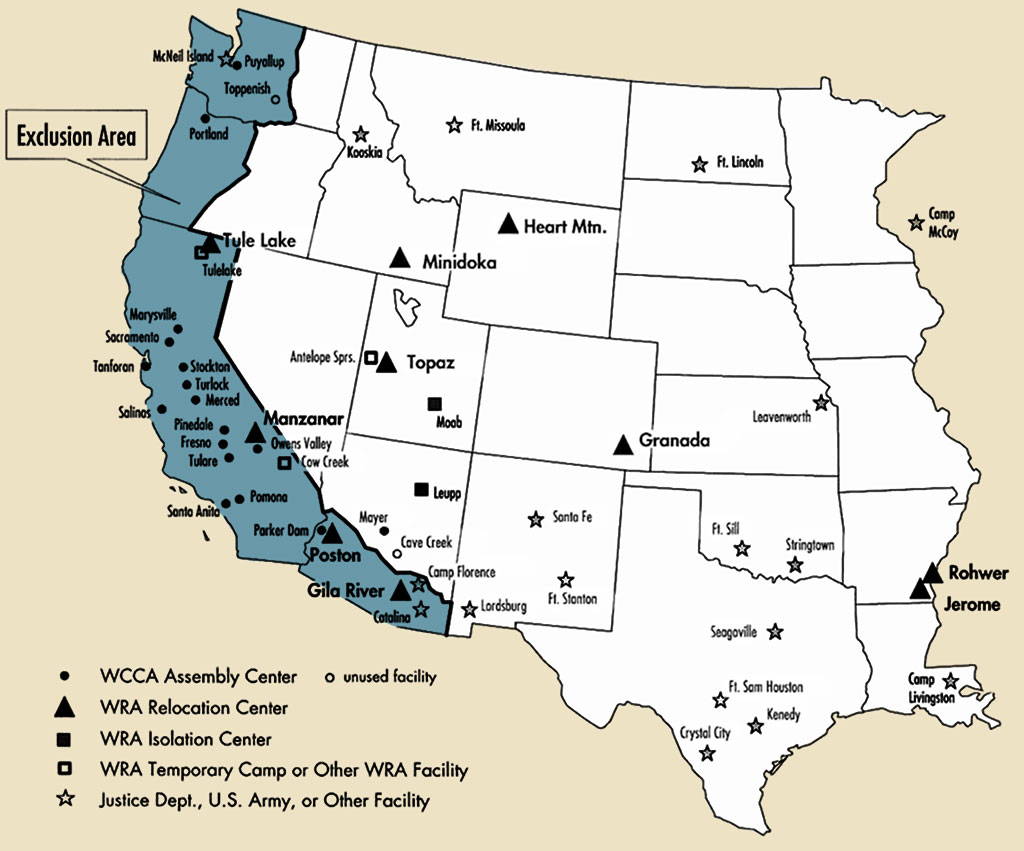
\includegraphics[width=1.0\linewidth]{figures/PioCrtInternmentMap.jpg}
    \caption{Caption}
    \label{fig:internment_map}
\end{figure}

Aside from the importance of understanding the losses to internees, Japanese Internment can also serve as an interesting natural experiment through the involuntary nature of the experiences of internees. One question asked by previous economic literature is the extent that locations in which people live affect their economic outcomes such as upward mobility or earnings. It is difficult to provide an unbiased causal estimate because households usually have a large degree of choice in where they live. Previous studies have used a variety of empirical strategies to separate out this causal effect including controlling for observable characteristics like education \cite{glaeser_cities_2001}, worker fixed-effects \citep{card_location_2021}, or through leveraging other exogenous placements of households like the Moving to Opportunity Experiment (\cite{ludwig_long-term_2013}, \cite{chetty_effects_2016}, etc). 

\begin{itemize}
\item
  Immigrant populations tend to concentrate near places of initial
  settlement
\item
  Integration/assimilation could be important for immigrant labor market
  outcomes

  \begin{itemize}
  
  \item
    \cite{damm_ethnic_2009}
  \end{itemize}
\item
  Evidence for Canadian Japanese internment having persistant effect on
  spatial Japanese distribution
\item
  \cite{chan_forced_2022}
\end{itemize}

\subsection{Initial Distribution of pre-war Japanese
Population}\label{initial-distribution-of-pre-war-japanese-population}

\begin{center}
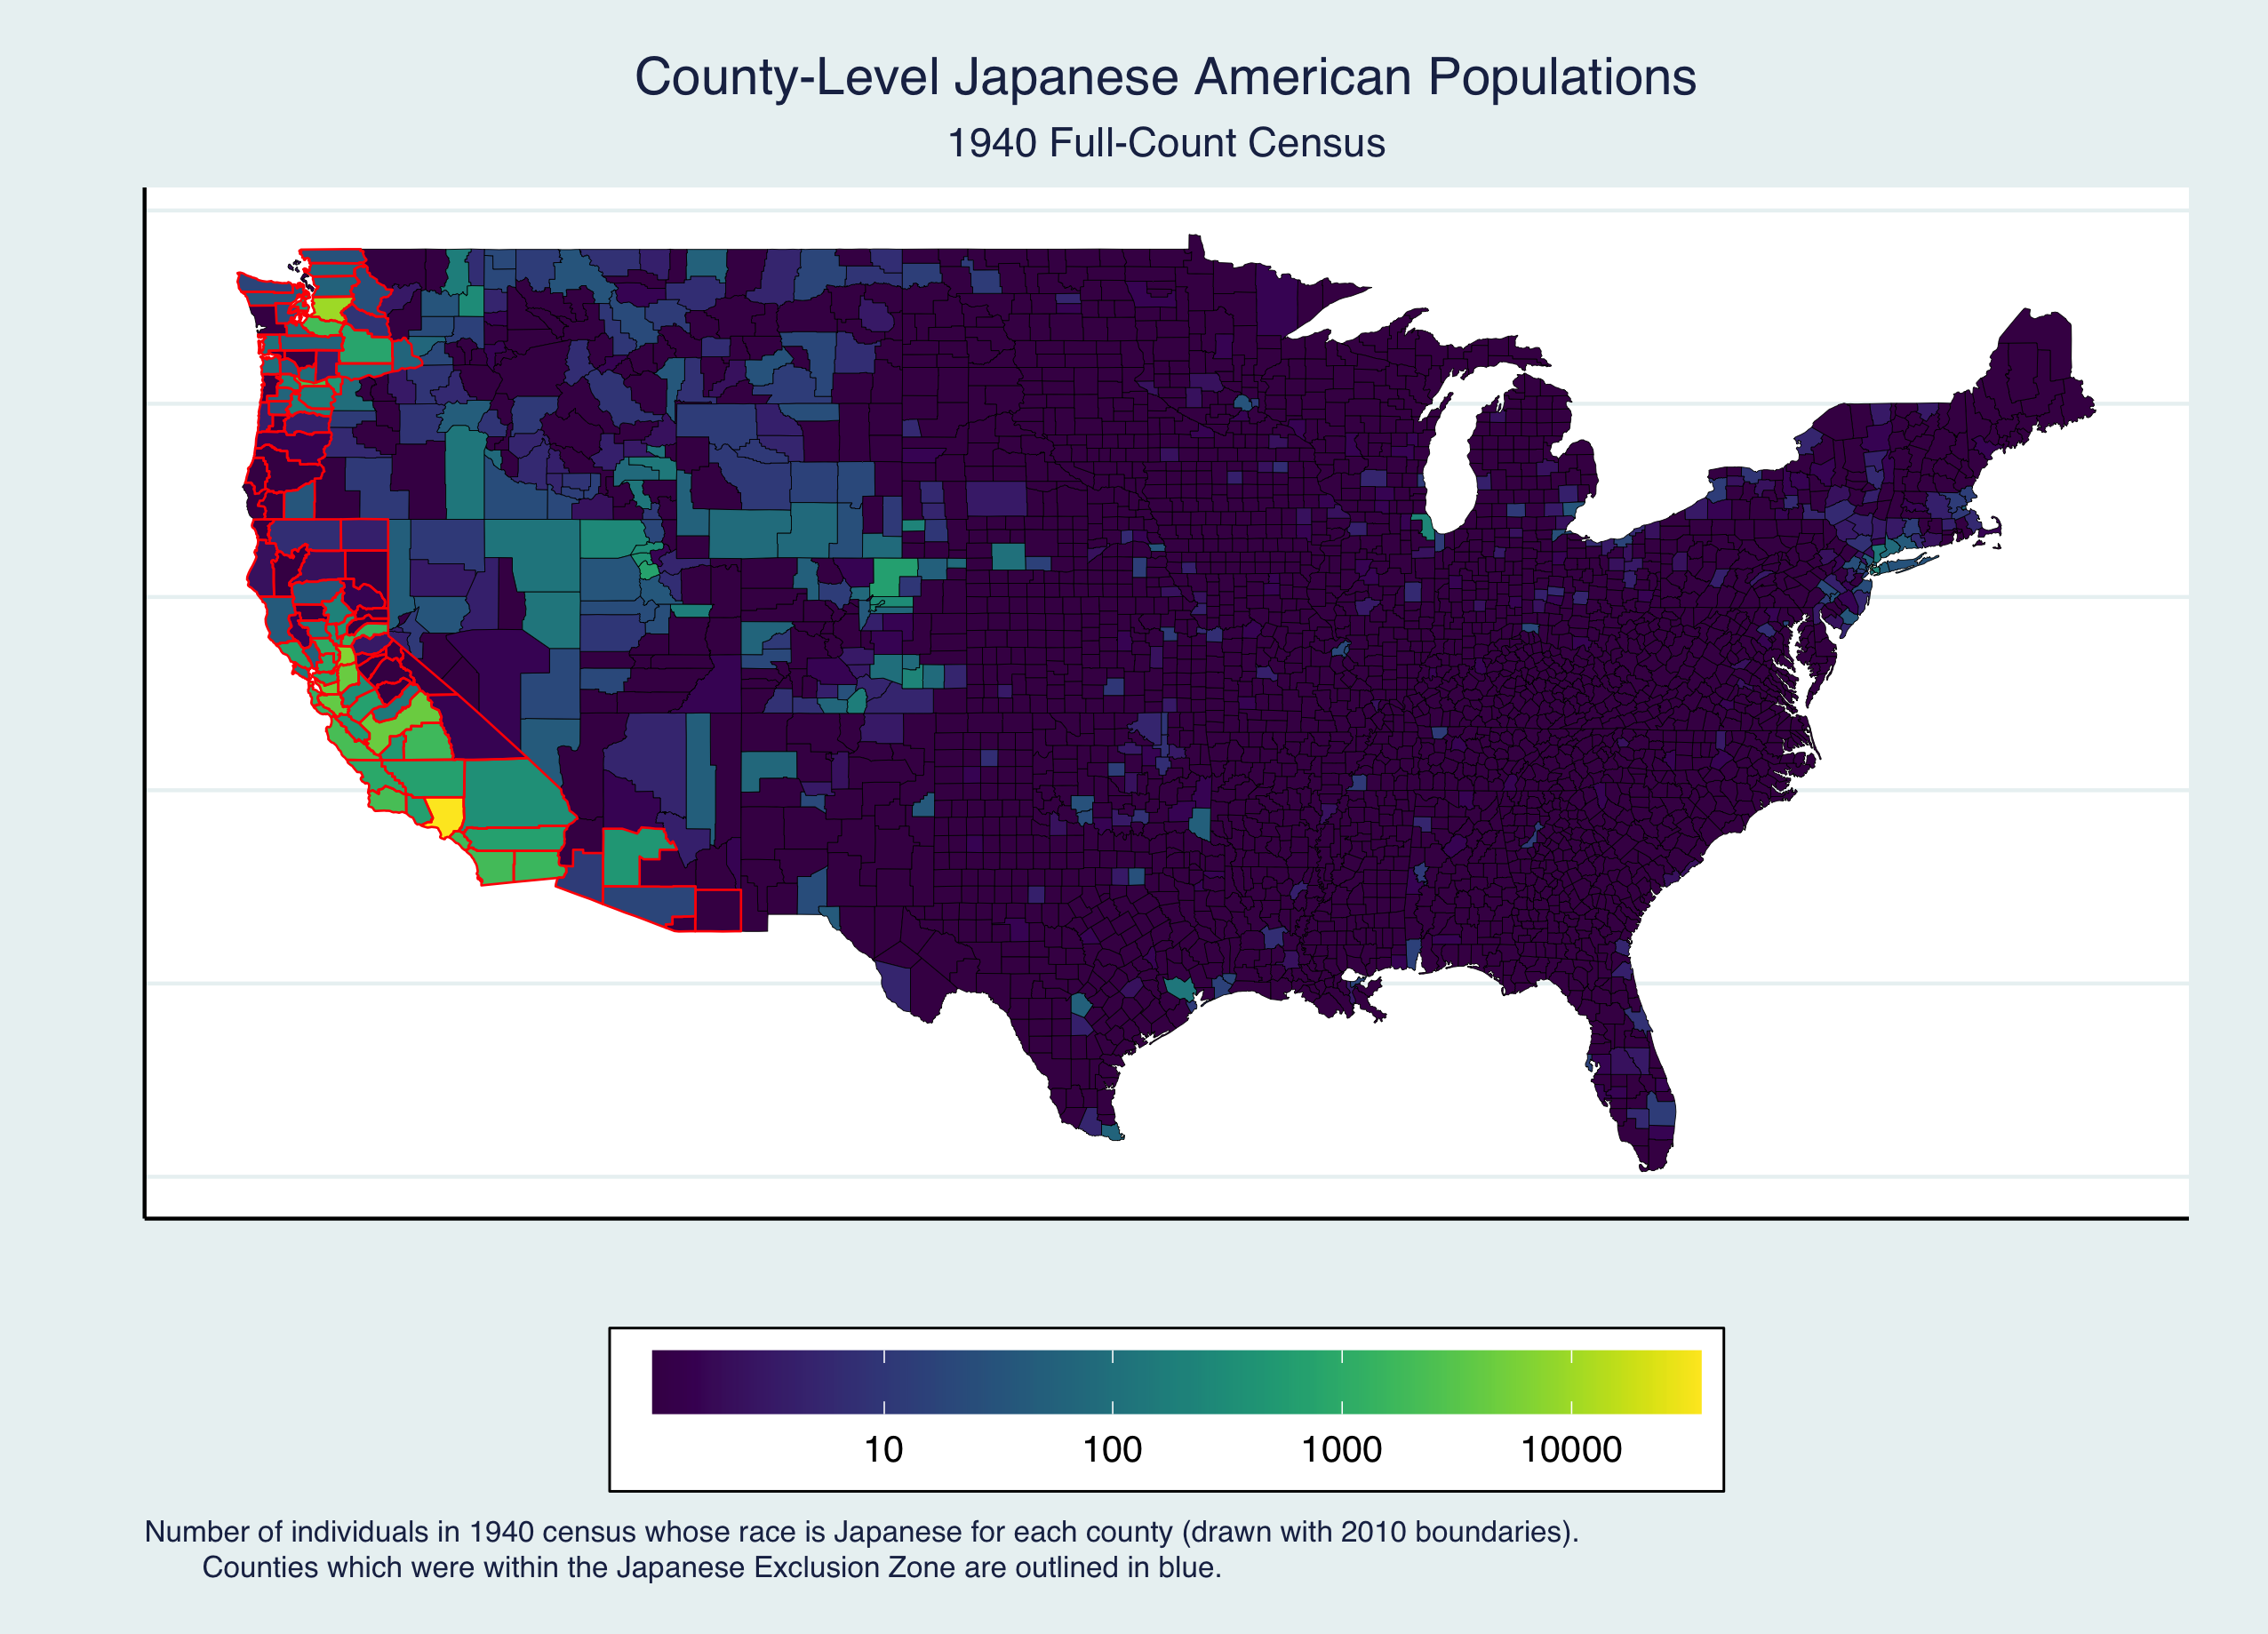
\includegraphics[width=1.0\textwidth]{figures/county_JAmap.png}
\end{center}

\subsection{Assignment of Internees to
Camps}\label{assignment-of-internees-to-camps}

\begin{center}
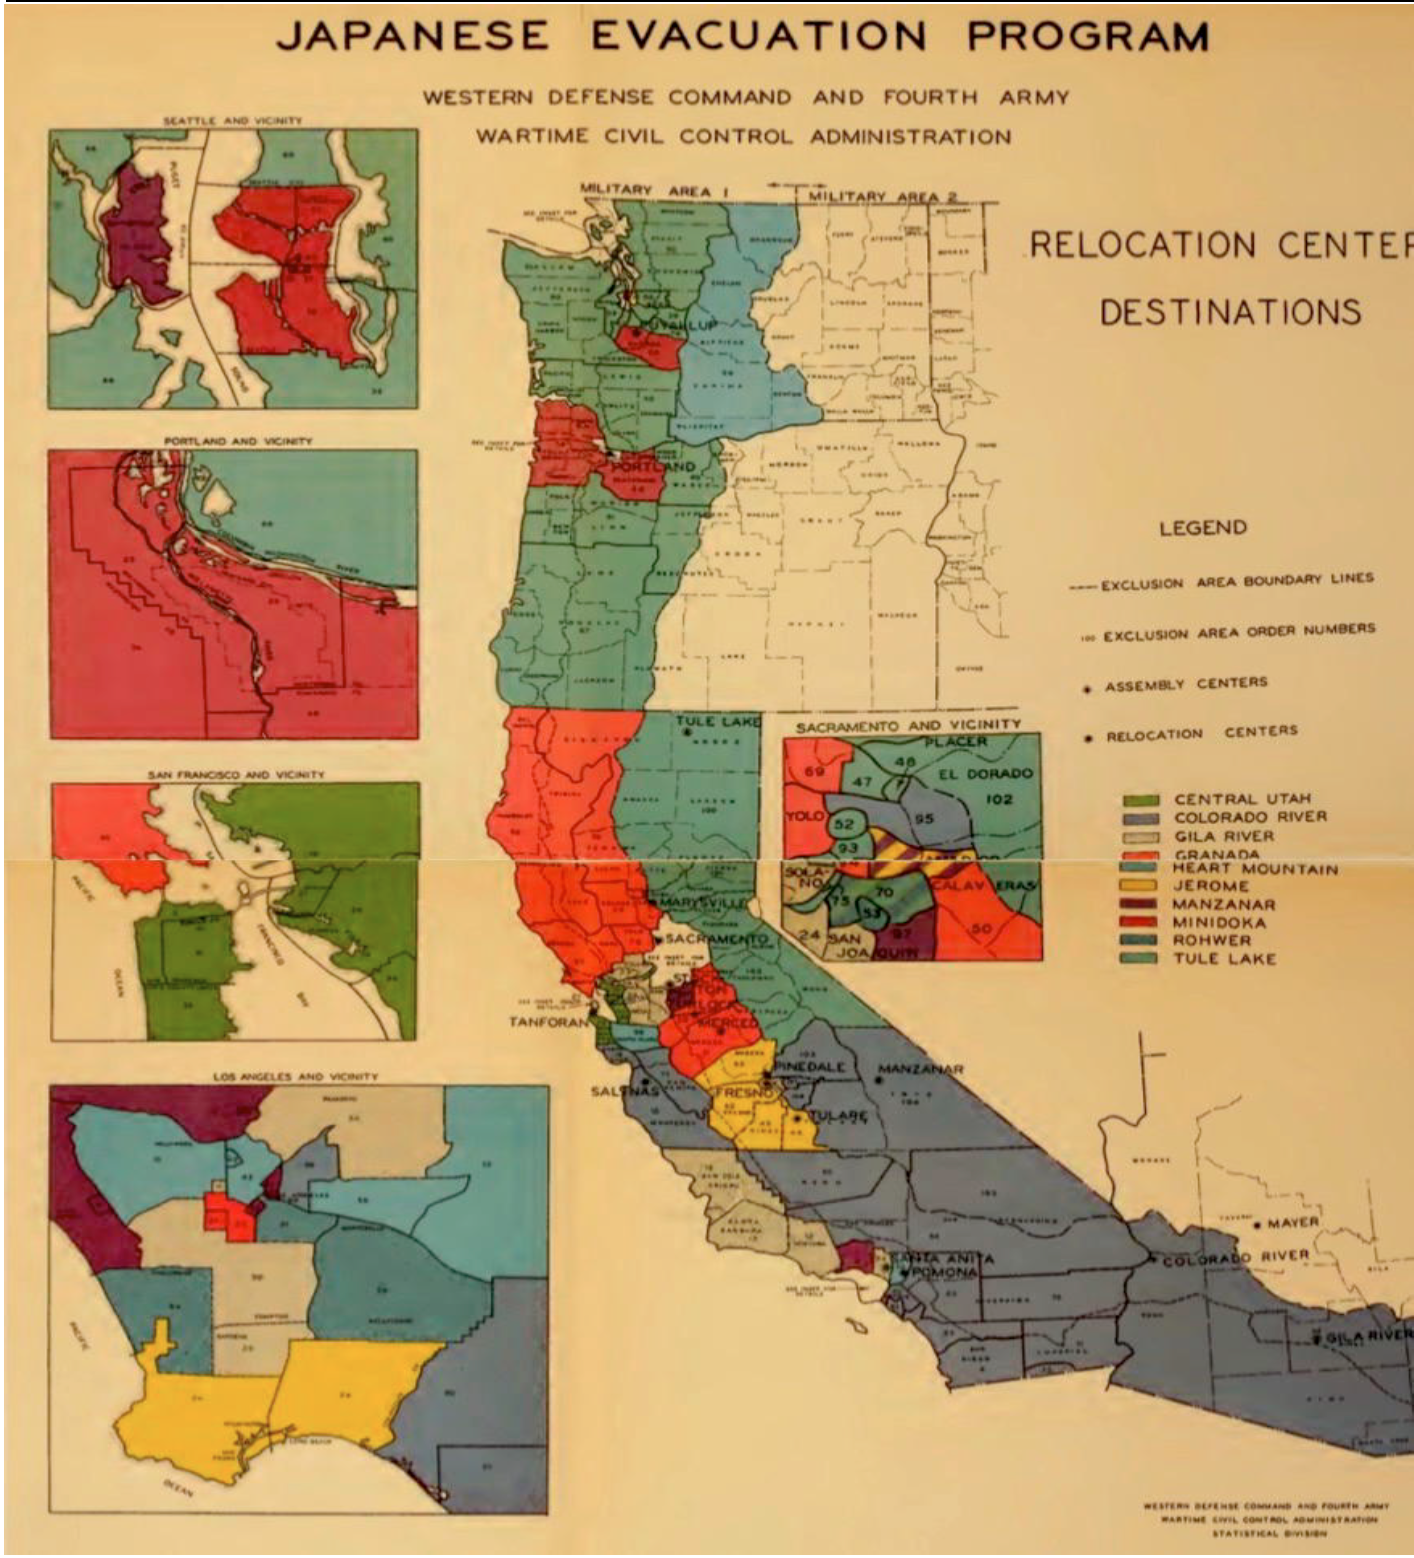
\includegraphics[width=1.0\textwidth]{figures/WRAzonesmap.png}
\end{center}

\begin{center}\rule{0.5\linewidth}{0.5pt}\end{center}

\section{Data}\label{data}


\subsection{Population and Migration}\label{population-and-migration}

For long-run migration data, I use the Decennial Census data provided by
the US Census Bureau via the
\href{https://usa.ipums.org/usa/index.shtml}{Integrated Public Use
Microdata Series} \citep{ruggles_ipums_2024}. The census
samples for which county locations are available include the 1940, 1950,
1980, and 1990 1\% samples, the 1960 5\% sample, and the 1970 Form 2
Metro 1\% sample.

For the calculation of migration rates between counties, I define a
migrant as someone who reports that they either moved within the state,
between states, or that they were abroad five years ago (or in the past
1 year for 1960 respondants). This excludes people who report moving
within the same house, didn't report their previous location, or the
location is unknown.

\subsection{Geography}\label{geography}

\subsubsection{Historical County Borders}\label{historical-county-borders}

Although most county borders did not change much in the second half of
the 20th Century, there were counties which split, merged, or had name
changes which can make cross-decade comparisons difficult. For these
reasons, I choose to standardize the set of counties in my analysis to
the set of counties as they appear in the year 1990. To map historical
county-level data to 1990 county definitions, I implement the crosswalk
method by \cite{eckert_method_2020}. They overlay historical
county boundary shapefiles from \href{NHGIS}{https://www.nhgis.org/}
onto county boundaries for a specific target year (in this case 1990).
The sub-areas created by these overlays are used to calculate a set of
geographic weights which represent the fractions of a 1990 county's area
which were within the geographic areas of counties as they appear in
different decades (specifically the decades between and including 1940
to 1980). For my analysis, I take the crosswalk weights from the example
csv file for the end year 1990 which is published on the authors'
\href{https://github.com/liang-jack-a/EGLP_Crosswalk/tree/master}{github
repository}.

%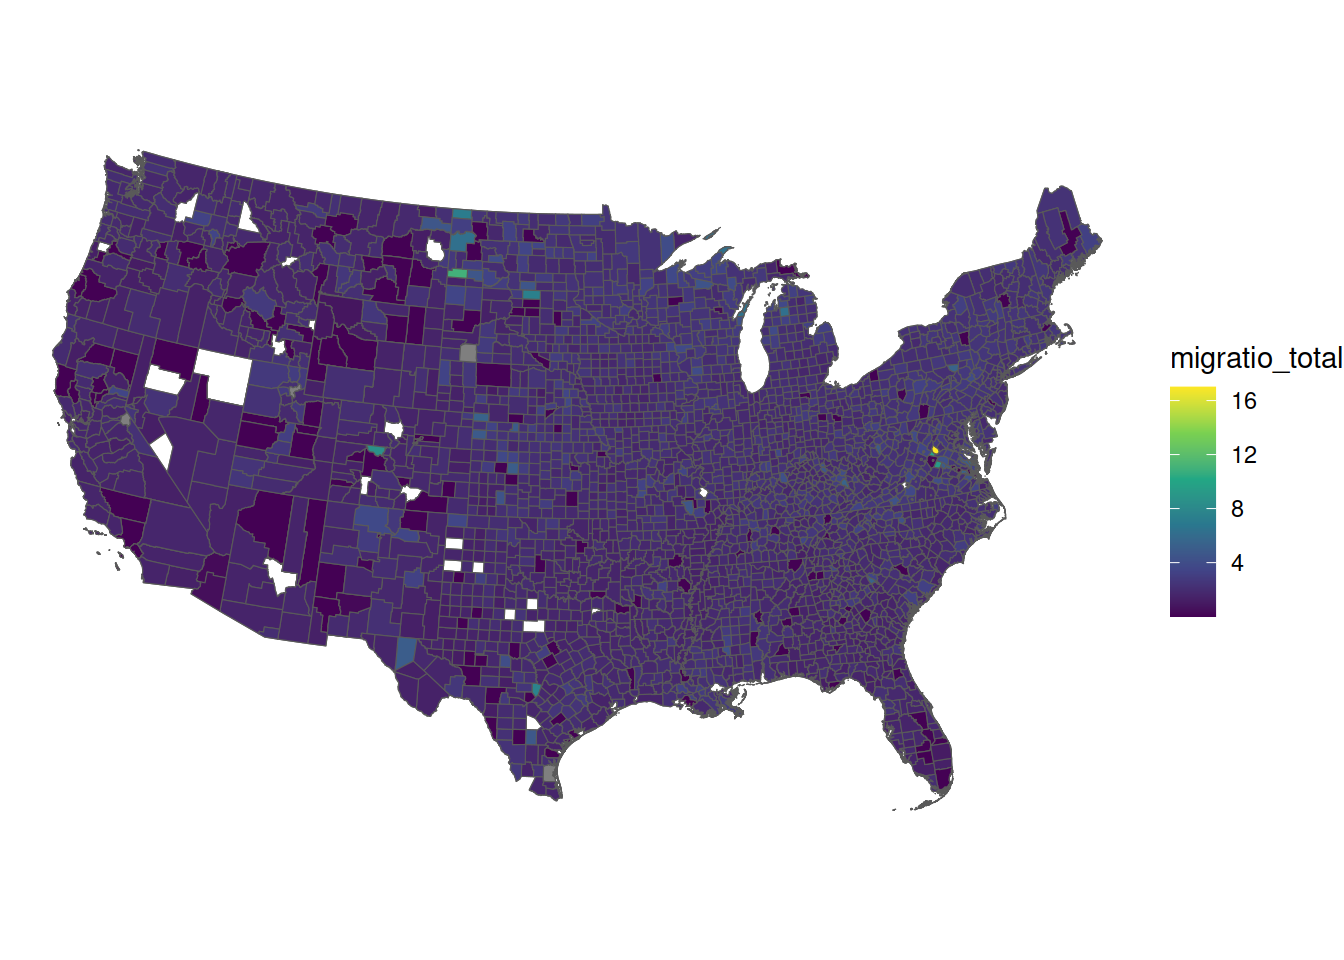
\includegraphics[width=1.0\textwidth]{main_files/figure-pdf/unnamed-chunk-1-1.pdf}

\subsubsection{Camp Locations}\label{camp-locations}

Locations for historical interment camp locations were archived by
\href{http://encyclopedia.densho.org/War_Relocation_Authority/\#Planning_the_Camps}{Densho
Encyclopedia} and downloaded in csv form via the
\href{https://www.arcgis.com/home/item.html?id=69183af8d45d4f46a9dc4eba99440891}{Behind
Barbed Wires story project}.

%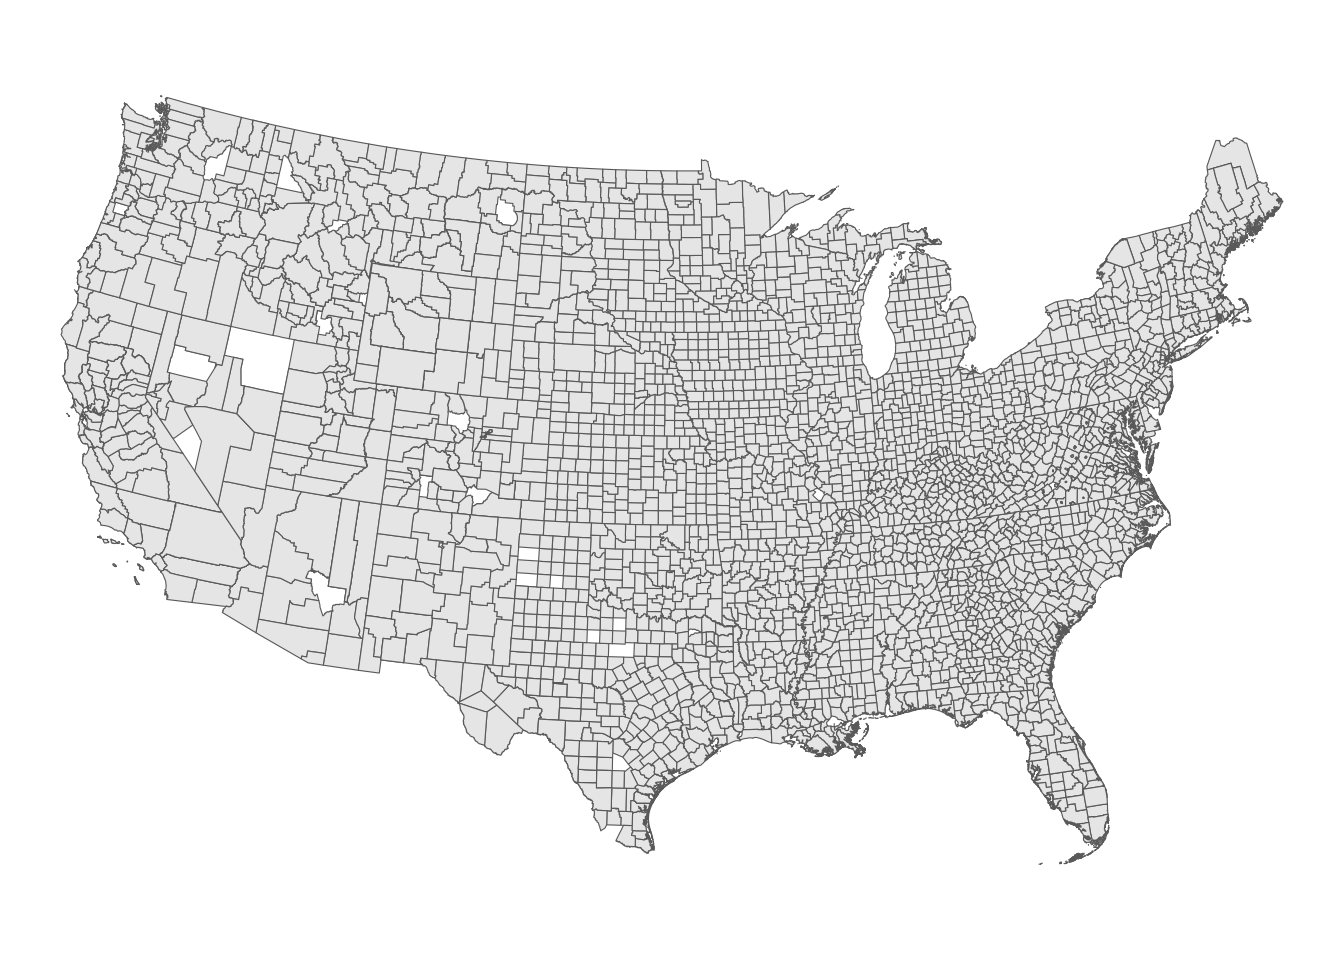
\includegraphics[width=1.0\textwidth]{main_files/figure-pdf/read-camplocations-1.pdf}

I calculate the straight line distances in meters between each 1950
county centroid to each camp location in QGIS with the
\texttt{Distance\ Matrix} tool using the Standard (N x T) distance
matrix setting.

\subsection{Historical counties
dataset}\label{historical-counties-dataset}

After narrowing down to counties which can be observed in each census
year and then translating the historical counties to 1990 county
boundaries, I am left with 3082 counties with observable migration rates
in 1940, 108 in 1950, 410 in 1960, 115 in 1970, 254 in 1980, and 290 in
1990.

My primary dataset is therefore a pooled-crossection with a total number
of 28 county-year level observations. Each observation represents an
individual county at a given year in time if it had the same borders as
it had in 1990.

The Census Bureau confidentiality standards state that public-use
microdata will cannot show report locations with populations of less
than 100,000 people. For this reason, many sparsely-populated counties
will be omitted from my sample because there are not enough observations
for the Census to report locations of individuals living there.

\phantomsection\label{cell-fig-comparesamplepops}
\begin{figure}[H]
\centering{
% 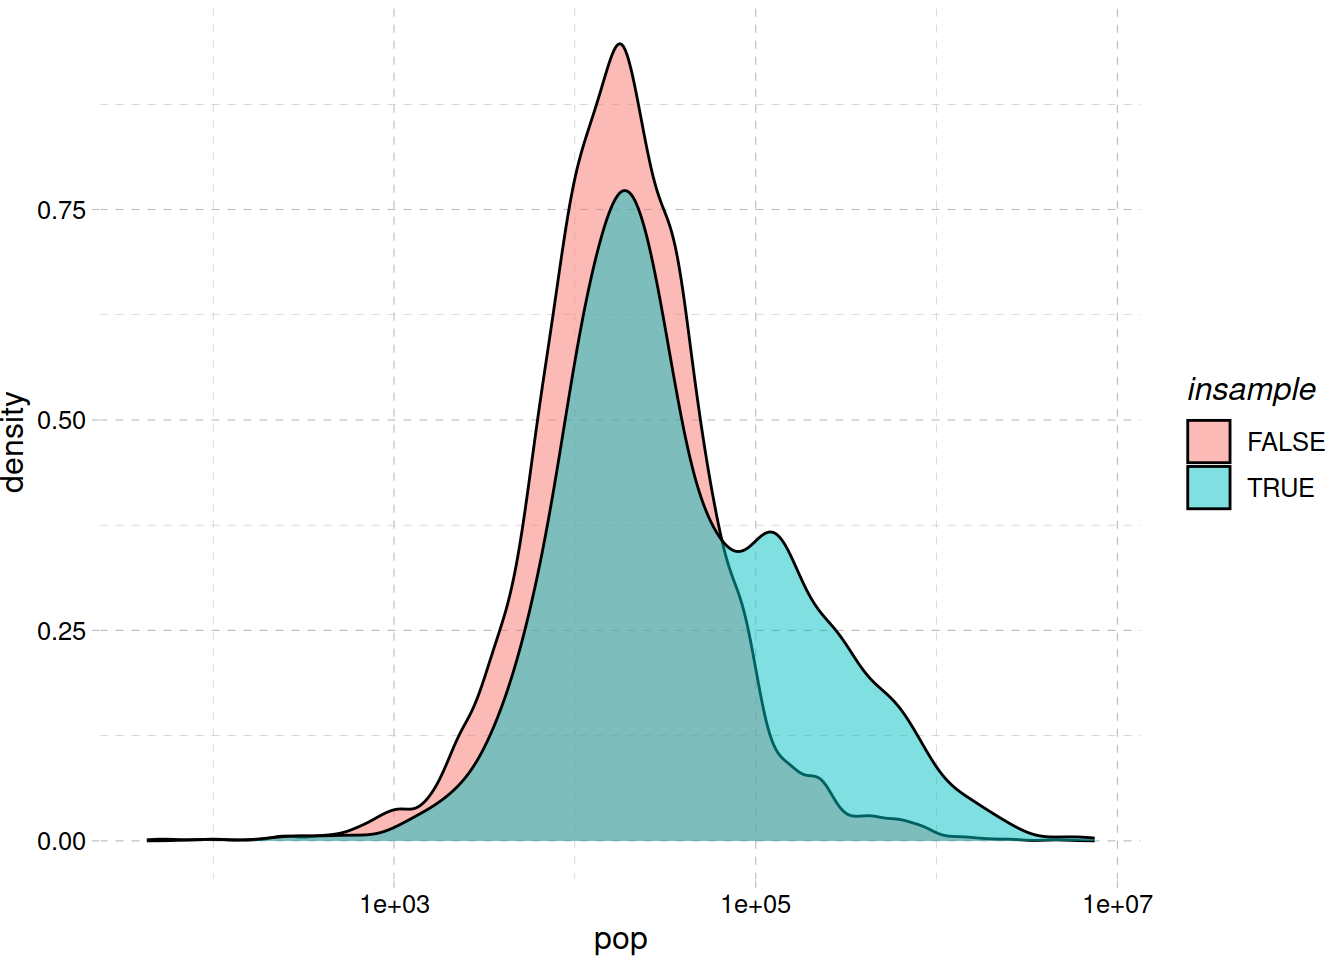
\includegraphics[width=1.0\textwidth]{figures/fig-comparesamplepops-1.pdf}
}
\caption{\label{fig-comparesamplepops}County-year level population
distributions}
\end{figure}%

The average population of the census-year observations in my sample is
133,000 while the average population for
crosswalked census-year observations outside my sample is
3,930,000. The fact that my sample is not
fully representative of all county sizes will be a challenge for the
external validity of my findings to extrapolate my results to smaller
counties for which I have less information on. However,
Figure~\ref{fig-comparesamplepops} shows that two different densities of
county-year populations observed in and out of the main sample have
similar shapes with the exception of a larger right-tail in the
in-sample density plot. This reflects the fact that counties with
populations of greater than 100,000 meet the Census Bureau's
confidentiality criteria, while data from smaller counties are subject
to stricter confidentiality measures.

\subsection{WRA first addresses}\label{wra-first-addresses}

\begin{itemize}

\item
  {\emph{The Evacuated People: A Quantitative Descripton}}
  \cite{krug_evacuated_1946}

  \begin{itemize}
  
  \item
    Final WRA report on ``State and Post Office Address of First
    Destination by Nativity, Prior January 1, 1945 and January 1, 1945
    and Later''
  \item
    Digitized and uploaded by \href{https://cooper-thomas.com/}{Cooper Thomas} via
    \href{https://data.world/infinitecoop/japanese-internment-camps}{data.world}
  \end{itemize}
\end{itemize}

\subsubsection{Map of Relocated Internees by
City}\label{map-of-relocated-internees-by-city}

\subsection{WRA internees}\label{wra-internees}

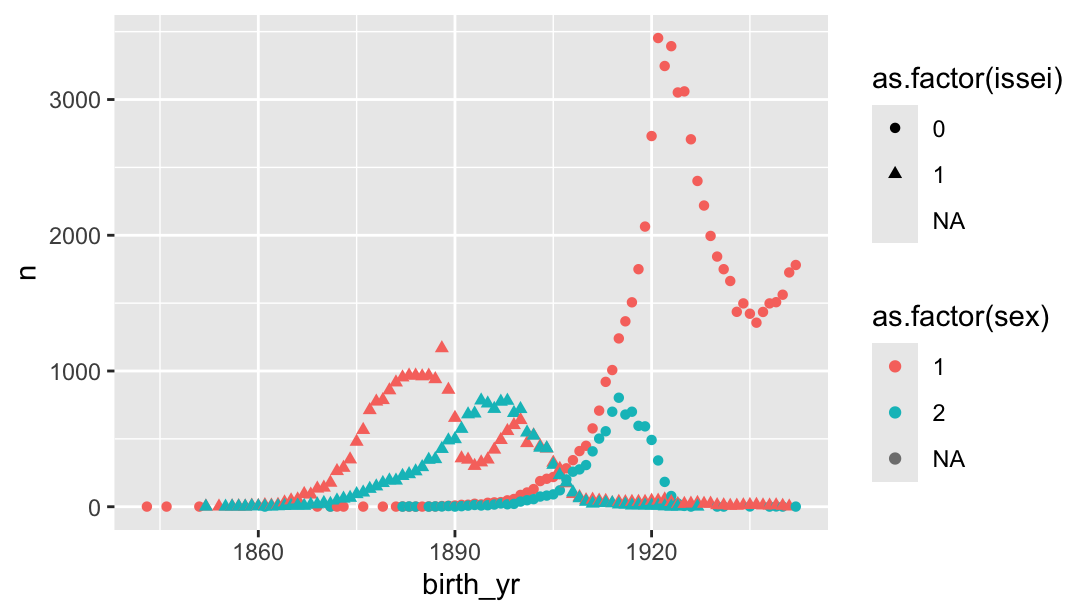
\includegraphics[width=1.0\textwidth]{figures/wra-internee-cohorts.png}

\subsection{IPUMS Census}\label{ipums-census}

\begin{itemize}

\item
  Decennial Census Data for years 1940, 1950, 1960, 1970, 1980, and 1990

  \begin{itemize}
  
  \item
    Via IPUMS USA \citep{ruggles_ipums_2024}
  \end{itemize}
\end{itemize}

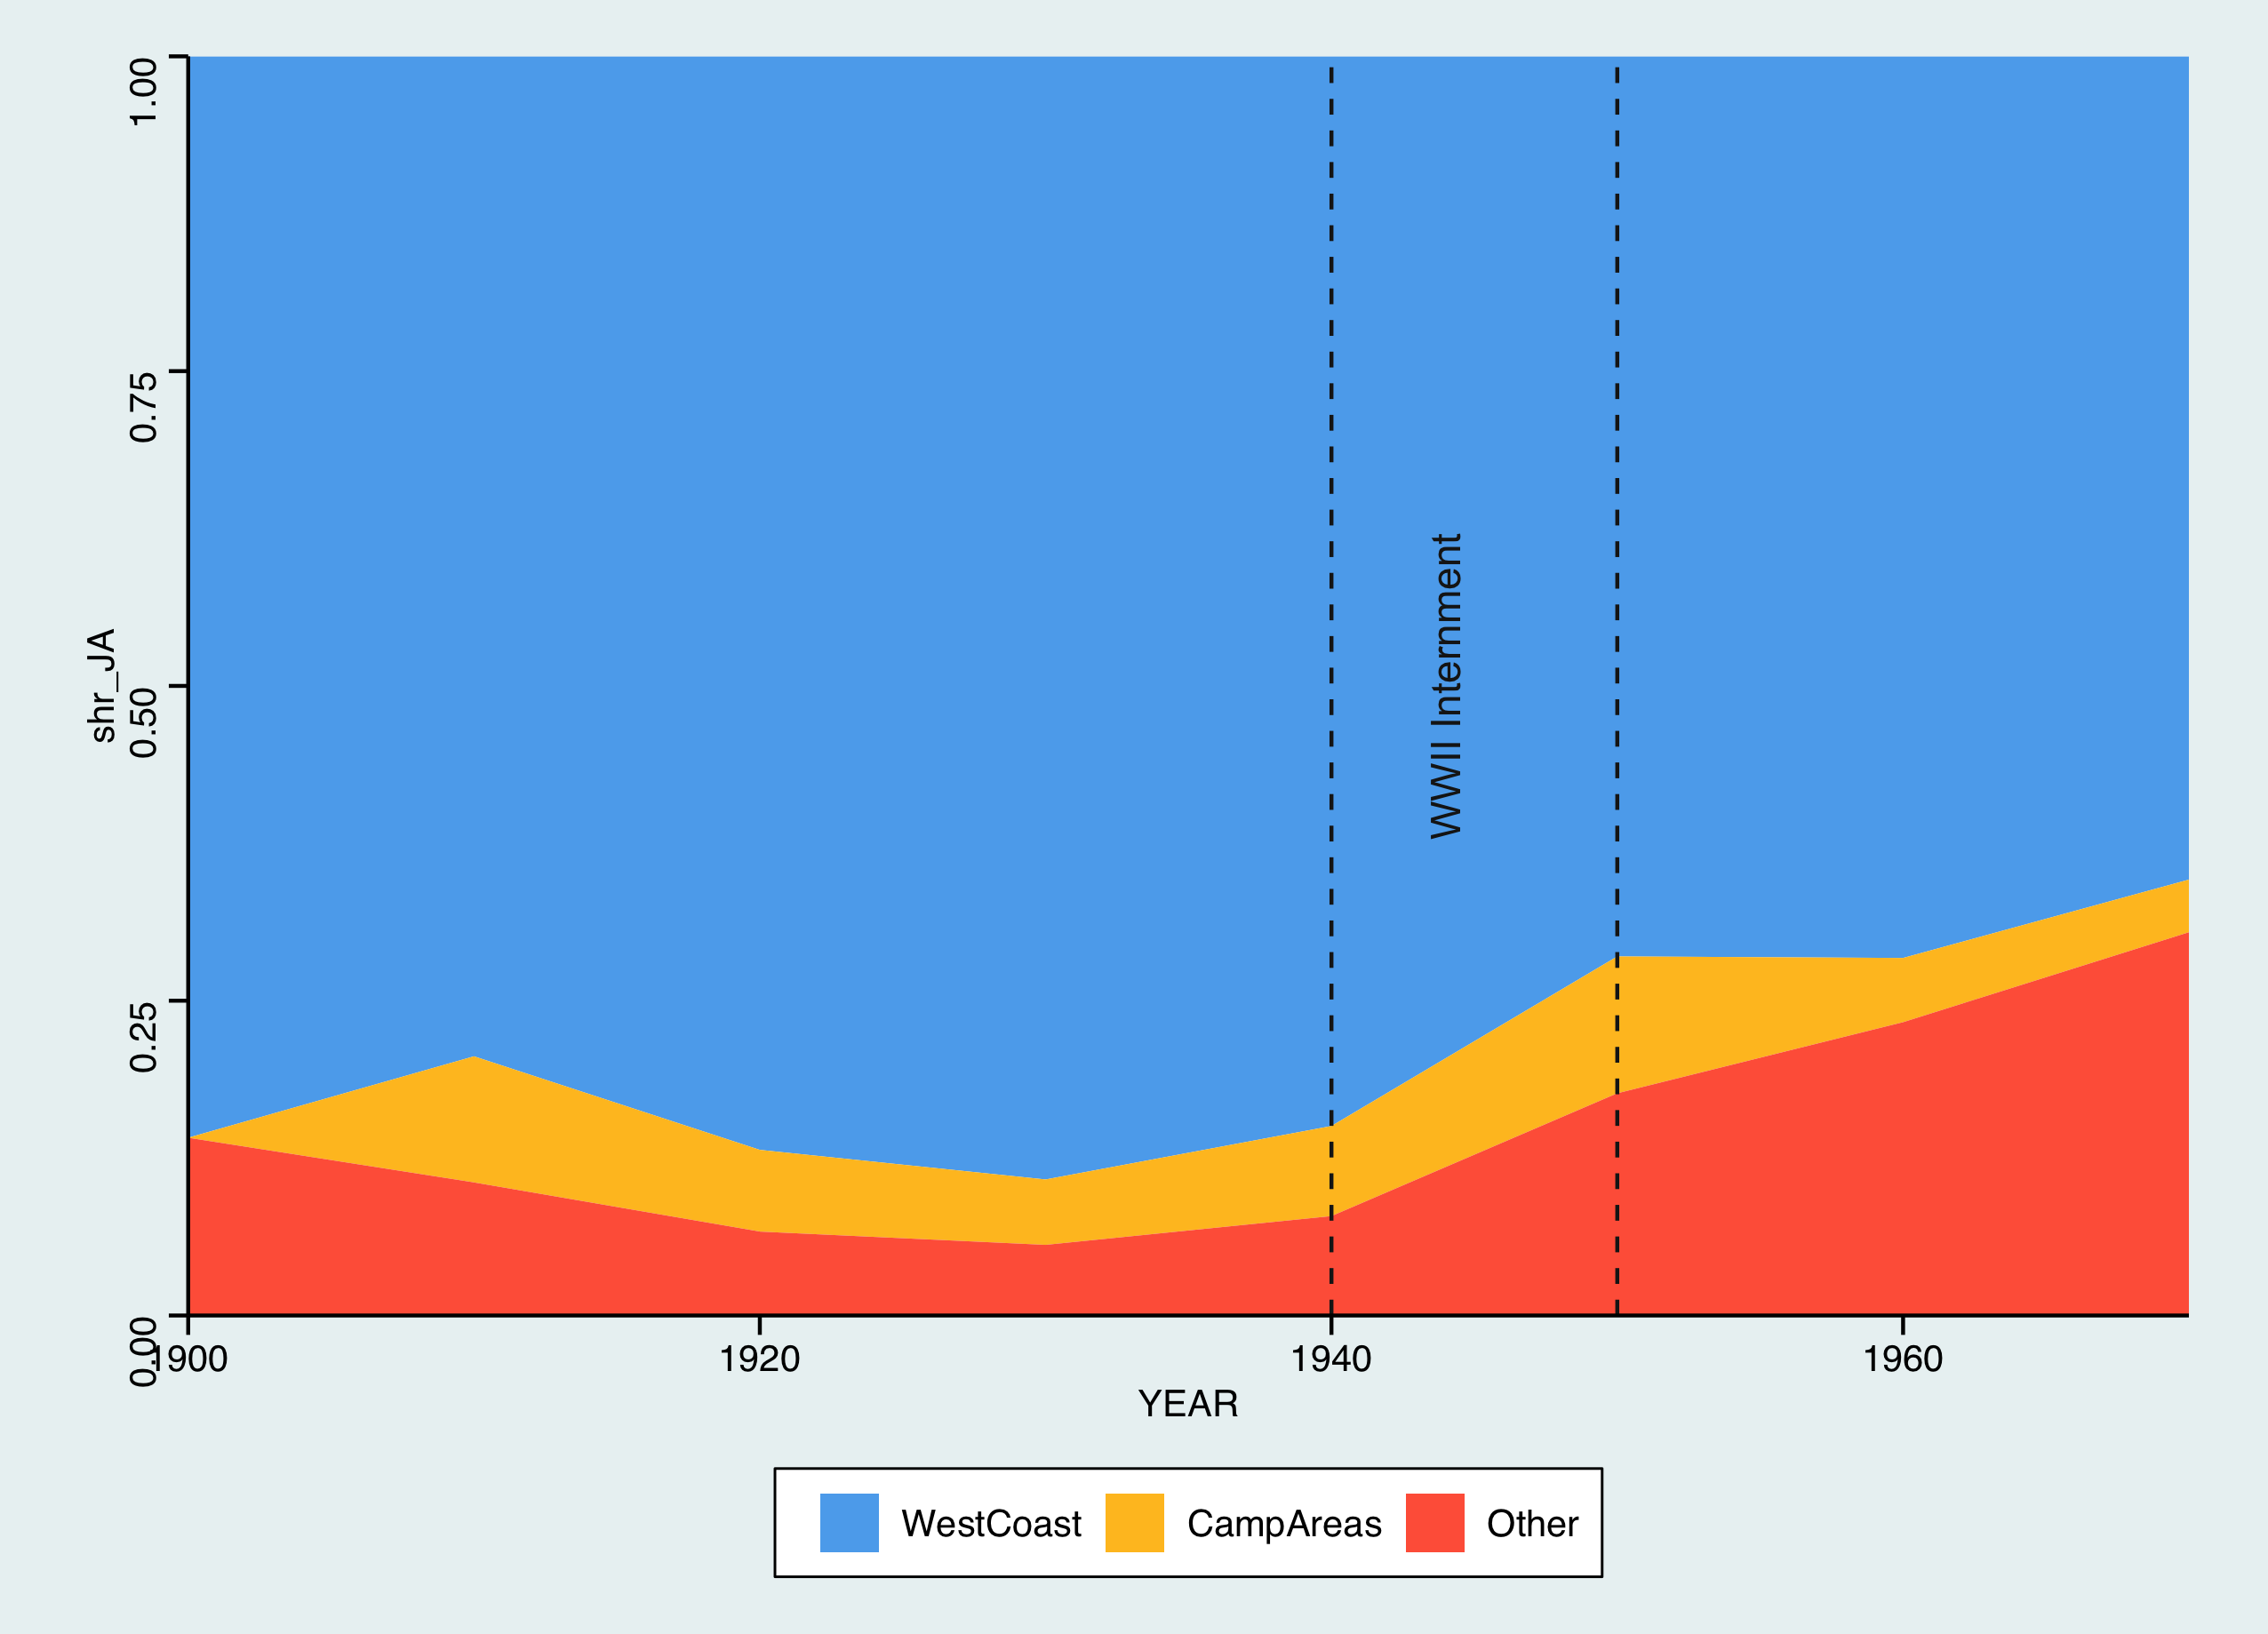
\includegraphics[width=1.0\textwidth]{figures/shareareaplot.png}

\subsection{NHGIS geo}\label{nhgis-geo}

\section{Methods}\label{methods}

\subsection{immigration on dist to
camps}\label{immigration-on-dist-to-camps}

\begin{equation}
    \frac{mig\_japn_{it}}{mig\_total_{it}} = \beta_0 + \beta_1 \min_{c\in C} Dist^{c\rightarrow i} 
+ \mathbb{X}_{ct} \gamma +  \epsilon_{ct}
\end{equation}

\subsubsection{within cont. US migration of japanese
americans}\label{within-cont.-us-migration-of-japanese-americans}

\subsubsection{new immigration from
japan}\label{new-immigration-from-japan}

\subsection{individual-level characteristics vs
internees?}\label{individual-level-characteristics-vs-internees}

\section{Results}\label{results}


% Table created by stargazer v.5.2.3 by Marek Hlavac, Social Policy Institute. E-mail: marek.hlavac at gmail.com
% Date and time: Wed, Sep 11, 2024 - 13:50:16
\begin{table}[!htbp] \centering 
  \caption{} 
  \label{} 
\begin{tabular}{@{\extracolsep{5pt}}lcccccc} 
\\[-1.8ex]\hline 
\hline \\[-1.8ex] 
 & \multicolumn{6}{c}{\textit{Dependent variable:}} \\ 
\cline{2-7} 
\\[-1.8ex] & \multicolumn{6}{c}{y} \\ 
\\[-1.8ex] & (1) & (2) & (3) & (4) & (5) & (6)\\ 
\hline \\[-1.8ex] 
 campclosest\_dist & $-$0.000$^{***}$ & $-$0.000 & $-$0.000$^{***}$ & $-$0.000$^{***}$ & $-$0.000$^{***}$ & $-$0.000$^{***}$ \\ 
  & (0.000) & (0.000) & (0.000) & (0.000) & (0.000) & (0.000) \\ 
  & & & & & & \\ 
 Constant & 0.002$^{***}$ & 0.002$^{**}$ & 0.003$^{***}$ & 0.006$^{***}$ & 0.004$^{***}$ & 0.005$^{***}$ \\ 
  & (0.0002) & (0.001) & (0.0003) & (0.001) & (0.001) & (0.0005) \\ 
  & & & & & & \\ 
\hline \\[-1.8ex] 
Observations & 3,056 & 108 & 407 & 115 & 252 & 289 \\ 
R$^{2}$ & 0.014 & 0.014 & 0.160 & 0.292 & 0.100 & 0.112 \\ 
Adjusted R$^{2}$ & 0.014 & 0.005 & 0.157 & 0.286 & 0.096 & 0.109 \\ 
Residual Std. Error & 0.005 (df = 3054) & 0.003 (df = 106) & 0.002 (df = 405) & 0.003 (df = 113) & 0.003 (df = 250) & 0.003 (df = 287) \\ 
F Statistic & 44.489$^{***}$ (df = 1; 3054) & 1.508 (df = 1; 106) & 76.862$^{***}$ (df = 1; 405) & 46.581$^{***}$ (df = 1; 113) & 27.652$^{***}$ (df = 1; 250) & 36.316$^{***}$ (df = 1; 287) \\ 
\hline 
\hline \\[-1.8ex] 
\textit{Note:}  & \multicolumn{6}{r}{$^{*}$p$<$0.1; $^{**}$p$<$0.05; $^{***}$p$<$0.01} \\ 
\end{tabular} 
\end{table} 


% Table created by stargazer v.5.2.3 by Marek Hlavac, Social Policy Institute. E-mail: marek.hlavac at gmail.com
% Date and time: Wed, Sep 11, 2024 - 13:50:20
\begin{table}[!htbp] \centering 
  \caption{} 
  \label{} 
\begin{tabular}{lcccccc} 
\\[-1.8ex]\hline 
\hline \\[-1.8ex] 
 & \multicolumn{6}{c}{\textit{Dependent variable:}} \\ 
\cline{2-7} 
\\[-1.8ex] & \multicolumn{6}{c}{y} \\ 
\\[-1.8ex] & (1) & (2) & (3) & (4) & (5) & (6)\\ 
\hline \\[-1.8ex] 
 campclosest\_dist & $-$0.000$^{***}$ & $-$0.000 & $-$0.000$^{***}$ & $-$0.000$^{***}$ & $-$0.000 & $-$0.000 \\ 
  & (0.000) & (0.000) & (0.000) & (0.000) & (0.000) & (0.000) \\ 
  & & & & & & \\ 
 ez & 0.002 & $-$0.001 & 0.002$^{**}$ & $-$0.002 & 0.002 & 0.001 \\ 
  & (0.001) & (0.003) & (0.001) & (0.001) & (0.002) & (0.001) \\ 
  & & & & & & \\ 
 campclosest\_dist:ez & 0.000$^{**}$ & 0.000 & 0.000 & 0.000$^{***}$ & 0.000$^{*}$ & 0.000$^{***}$ \\ 
  & (0.000) & (0.000) & (0.000) & (0.000) & (0.000) & (0.000) \\ 
  & & & & & & \\ 
 Constant & 0.001$^{***}$ & 0.001 & 0.002$^{***}$ & 0.004$^{***}$ & 0.001$^{*}$ & 0.002$^{***}$ \\ 
  & (0.0002) & (0.001) & (0.0003) & (0.001) & (0.001) & (0.001) \\ 
  & & & & & & \\ 
\hline \\[-1.8ex] 
Observations & 3,056 & 108 & 407 & 115 & 252 & 289 \\ 
R$^{2}$ & 0.045 & 0.040 & 0.272 & 0.560 & 0.280 & 0.292 \\ 
Adjusted R$^{2}$ & 0.044 & 0.012 & 0.267 & 0.548 & 0.272 & 0.284 \\ 
Residual Std. Error & 0.005 (df = 3052) & 0.003 (df = 104) & 0.002 (df = 403) & 0.002 (df = 111) & 0.003 (df = 248) & 0.003 (df = 285) \\ 
F Statistic & 47.907$^{***}$ (df = 3; 3052) & 1.427 (df = 3; 104) & 50.239$^{***}$ (df = 3; 403) & 47.128$^{***}$ (df = 3; 111) & 32.185$^{***}$ (df = 3; 248) & 39.131$^{***}$ (df = 3; 285) \\ 
\hline 
\hline \\[-1.8ex] 
\textit{Note:}  & \multicolumn{6}{r}{$^{*}$p$<$0.1; $^{**}$p$<$0.05; $^{***}$p$<$0.01} \\ 
\end{tabular} 
\end{table} 


\section{Conclusion}\label{conclusion}


\bibliography{bibliography}

\end{document}
